% Template by - Santiago Morante
% Slightly modified by - David Estevez

\documentclass[11pt,a4paper,twoside]{book}
\usepackage{authoraftertitle}
\usepackage[pdftex]{hyperref}
\usepackage{graphicx}
\usepackage[english]{babel}
\usepackage[utf8]{inputenc}
\usepackage{fancyhdr}
\usepackage{invuc3mlib}
\usepackage{url}
%\usepackage{apacite}
\usepackage[nottoc,notlof,notlot]{tocbibind}%was commented out.
\usepackage{palatino}
\usepackage[Lenny]{fncychap}
\usepackage[font=small,format=plain,labelfont=bf,up,textfont=it,up]{caption}
\usepackage{colortbl}
\usepackage{indentfirst}
\usepackage{hhline}
\usepackage{mathtools}
\usepackage{amsmath}
\hypersetup{  
    pdftitle={Master Thesis - Author},
    pdfsubject={Master Thesis - Author},
    pdfauthor={Author},
    pdfkeywords={keyword1} {keyword2},
    colorlinks,
    citecolor=black,
    filecolor=black,
    linkcolor=black,
    urlcolor=black, } 

\usepackage[twoside]{geometry}
\geometry{twoside, bindingoffset=1cm, papersize={210mm,297mm}, total ={135mm, 220mm}, includefoot, includehead}

\setlength{\topmargin}{0cm} 
\setlength{\headsep}{8mm}
\setlength{\marginparwidth}{20mm} \setlength{\evensidemargin}{4mm} \setlength{\oddsidemargin}{20mm}
\newcommand{\clearemptydoublepage}{\newpage{\pagestyle{empty}%
\cleardoublepage}}

% Define a command for comments
\usepackage{color}
\newcommand{\comment}[1]{\textbf{\color{cyan} #1}}
\newcommand{\warning}[1]{\textbf{\color{red} #1}}

\usepackage[english]{babel}

\begin{document}
	\title{\textbf{\warning{Folding Clothes with a Robotic Slave}}}
	\author{David Estevez Fernandez}
	\tutor{Juan G. Victores}
  	\stutor{Carlos Balaguer}

        \primerjurado{Dr./Dra.}
        \segundojurado{Dr./Dra.}
        \thirdreader{Dr./Dra.}
		
    \dedicate{
\begin{flushright}
   \warning{``It's better to have loved and lost than to have to do forty pounds of laundry a week.''\\    
    Laurence J. Peter}
\end{flushright}
    }

    	\beforepreface

    \prefacesection{Acknowledgments}
   Thanks to all ...

  	\prefacesection{Resumen}
   	 
Esta tesis desarrolla ...

		\prefacesection{Abstract}
This thesis develops ...

	\cleardoublepage
    	\afterpreface

	\pagestyle{fancyplain}
	\renewcommand{\chaptermark}[1] %
	{\markboth{#1}{\thechapter\ #1}}
	\renewcommand{\sectionmark}[1]%
	{\markright{\thesection\ #1}}
	\lhead[\fancyplain{}{\bfseries\thepage}]
	{\fancyplain{}{\bfseries\rightmark}}
	\rhead[\fancyplain{}{\bfseries\leftmark}] {\fancyplain{}{\bfseries\thepage}}
	\cfoot{}
	
	\chapter{Introduction}
\label{introduction}

\section{Introduction}
\label{intro_introduction}

\section{Objectives}
\label{intro_objectives}

\section{Structure}
\label{intro_structure}
	\chapter{State of the Art}
\label{state_of_the_art}

In this chapter, the current state of the art regarding garment folding is presented. Different approaches when working with garments can be found in the literature, and they will be described in this chapter.

Some approaches use 3D computer vision algorithms to create models of the garments or to fit captured gament data to a predefined model. These garment models are used then to apply folding algorithms or to select the best points for manipulation. Some of these models are borrowed from the Computer Graphics community, where garment representation and simulation has been widely studied to achieve realistic clothes behavior in Computer Graphics scenes. This will be covered in section \ref{sota:garment_model_based}.

In other approaches, the problem of garment folding is solved through robot interaction with the garment. By regrasping and changing the garment configuration, the garment category and current pose is detected, and the garment can be led to a target pose. These approaches will be seen in section \ref{sota:garment_manipulation_based}.

Finally, the european project CloPeMa (Clothes Perception and Manipulation), devoted to perception and manipulation of fabric, textiles and garments, is described. Their research most relevant to this thesis is explained in the last section \ref{sota:clopema}.

\section{Garment Modeling-Based Approaches}
\label{sota:garment_model_based}
A significant amount of work conducted in this topic has been focused on modeling the different garment categories for both unfolded, extended garments and for grasped garments. The computer graphics community has also contributed with extensive work on the specifics of clothes modeling due to their need for realistic representation of fabrics and garments. A review of these modeling methods can be found in \cite{Chen2009}. 

Kita et al. propose a method that uses a deformable model to calculate the state of hanging clothes based on 3D observed data \cite{Kita2004, Kita2009}. This calculation is performed by generating a set of candidate shapes predicted by physical simulations of hanging clothes and later comparison of them with the observed data. To fit the observed 3D data better, each generated shape is further deformed and the shape that is more consistent with the observed data is selected. 

\begin{figure}[thpb]
    \centering
    \includegraphics[width=0.95
    \textwidth]{figures/SOTA_Kita_2009.png}
    \caption{\comment{(Kita thing)}}
    \label{fig:SOTA_Kita_2009}
\end{figure}

Miller et al. present an approach to modeling the clothes when already spread out on a flat surface in \cite{Miller2011}. A series of parametrized shape models are proposed, each clothing category having its own model. Garment variability is solved through variation of those parameters. Once the garment has been modeled with their method, a preprogrammed folding sequence can be performed.

%\begin{figure}[thpb]
%    \centering
%    \includegraphics[width=0.6
%    \textwidth]{figures/SOTA_Miller_2011.png}
%    \caption{\comment{(Miller thing - add more models)}}
%    \label{fig:SOTA_Miller_2011}
%\end{figure}

\begin{figure}[htbp]
	\centering
    \begin{subfigure}[l]{0.49\textwidth}
        \centering
    	\includegraphics[width=\textwidth]
    	{figures/SOTA_Miller_2011.png}
        \end{subfigure}
        ~
        \begin{subfigure}[r]{0.49\textwidth}
	        \centering
    		\includegraphics[width=\textwidth]
    		{figures/SOTA_Miller_2011-2.png}
		\end{subfigure} 
    	\caption{\comment{(Miller thing)}}
    	\label{fig:SOTA_Miller_2011}
\end{figure}

A method for classifying and estimating the poses of deformable objects is presented in \cite{Li2014ICRA}. This method consists in creating a training set of deformable objects by off-line simulation of different garments, extracting depth images from different points of view. Then, a codebook is built for a set of different poses of each deformable object by extracting features from the dataset and applying sparse coding and dictionary learning. With this codebook, classifying deformable objects on different categories and estimating their current pose is possible, for later regrasping or folding the garment.

The previous method was improved in \cite{Li2014IROS}, by extracting the features directly from the 3D data, dividing the hanging garment in different cells via layers, rings and sectors of the bounding cylinder. Each of the sectors becomes a binary feature, using the Signed Distance Function to check if the cell is inside the voxel where the center of the cell belongs, and is then arranged in a feature vector. A Hamming distance, whose weights are learned from the simulated dataset merged with some models reconstructed from real word Kinect point clouds, is used to estimate the object category and pose given an input reconstructed mesh model.

\begin{figure}[thpb]
    \centering
    \includegraphics[width=\textwidth]{figures/SOTA_Li_2014-2.png}
    \caption{\comment{(Li thing - two figures available)}}
    \label{fig:SOTA_Li_2014}
\end{figure}

\section{Garment Manipulation-Based Approaches}
\label{sota:garment_manipulation_based}
Clothing article manipulation is another field in which extensive work has been done. Based on the previous recognition algorithm, Li presents in \cite{Li2015ICRA} a method for unfolding deformable objects with a bi-manipulator robot. With this method, the robot is capable of taking a clothing article from an unknown state to a known state by iterative regrasping, detecting the most suitable grasping points in each state to achieve its goal. For locating the most suitable grasping points, the 3D point cloud obtained by the robot is matched to the mesh model, that incorporates the information about the best regions to grasp in order to unfold the garment.

\begin{figure}[thpb]
    \centering
    \includegraphics[width=\textwidth]{figures/SOTA_Li_2015.png}
    \caption{\comment{(Li thing - two figures available)}}
    \label{fig:SOTA_Li_2015}
\end{figure}

The method introduced by Cusumano-Towner et al. in \cite{Cusumano-Towner2011} allows a bi-manipulator robot to identify a clothing article, estimate its current state and achieve a desired configuration, generalizing to previously unseen garments. For that purpose, the robot uses a Hidden Markov Model (HMM) throughout a sequence of manipulations and observations, in conjunction with a relaxation of a strain-limiting finite element model for cloth simulation that can be solved via convex optimization.

\begin{figure}[thpb]
    \centering
    \includegraphics[width=\textwidth]{figures/SOTA_Cusumano_PR2.png}
    \caption{\comment{(Cusumano thing)PR2}}
    \label{fig:SOTA_Cusumano_2011}
\end{figure}

Osawa et al. propose in \cite{Osawa2006} a method to unfold garments in order to classify them. It consists in alternatively regrasping clothing and expanding them using a two-arms manipulator. The garment is grasped with one arm and the lowest point is located by rotating the piece of clothing, which is used as a grasping point for the other arm. If the garment has any fold when extended, it is placed over a flat surface to repeat this process util the the garment is fully spread out.

To detect the best grasping points for a clothing article, Ramisa \cite{Ramisa2012} performs the identification in a single step, even with highly wrinkled clothes. This detector is based in a Bag of Features detector, using as input a combination of appearance and 3D geometric features.

The most similar work we can find in the related literature is the method for unfolding clothes presented by Willimon et al. in \cite{Willimon2011}. Their method, which also focuses in clothes unfolding prior to automated folding, use several features obtained from a depth image, such as peak regions and corners location, to determine the location and orientation most suitable for interaction with the garment. Two main steps are performed: first, the clothing article is flattened using RGB information from the camera and, then, depth information is used to extract the features used to estimate how to unfold the garment.

\section{CloPeMa European Project}
\label{sota:clopema}

CloPeMa\footnote{\url{http://www.clopema.eu/}} is a recent EU-FP7 research project (2012-2015) whose objective is to advance the state of the art in perception and manipulation of fabric, textiles and garments.

\begin{figure}[thpb]
    \centering
    \includegraphics[width=0.7
    \textwidth]{figures/SOTA_CloPeMa_logo.png}
    \caption{\comment{(Nice description)}}
    \label{fig:SOTA_CloPeMa_logo}
\end{figure}

 As part of the CloPeMa project, a method to detect single folds has been presented by Mariolis et al. in \cite{Mariolis2013, Mariolis2015}. In order to detect such folds, a database of unfolded clothes templates is built in the first place. These templates are later used to perform a shape matching between the folded garment shape, obtained by the camera, and the unfolded garment model. This process is iterative, and the initial results are feedbacked to adapt the model for a better fit. 

\begin{figure}[thpb]
    \centering
    \includegraphics[width=\textwidth]{figures/SOTA_Mariolis_2015.png}
    \caption{\comment{(Mariolis thing)}}
    \label{fig:SOTA_Mariolis_2015}
\end{figure}

Stria et al. propose in \cite{Stria2014, Stria2014IROS} a polygon-based model for clothes configuration recognition using the estimated position of the most important landmarks in the clothing article. Once identified, these landmarks can be used for automated folding using a robotic manipulator. The clothes contour is extracted from a RGB image and processed using a modified grabcut algorithm and dynamic programming methods are used to fit it to the polygonal model.

\begin{figure}[thpb]
    \centering
    \includegraphics[width=\textwidth]{figures/SOTA_Stria_2014-2.png}
    \caption{\comment{(Stria thing - two figures)}}
    \label{fig:SOTA_Stria_2014}
\end{figure}


Doumanoglou et al. follow in \cite{Doumanoglou2014ECCV} an approach based on Active Random Forests to recognize clothing articles from depth images. This classifier allows the robot to perform actions to collect extra information in order to disambiguate the current hypotheses, such as changing the viewpoint. In \cite{Doumanoglou2014ICRA} they extend this approach to detect the optimal grasping points to unfold the garment.


\begin{figure}[thpb]
    \centering
    \includegraphics[width=0.9
    \textwidth]{figures/SOTA_Doumanoglou_2014.png}
    \caption{\comment{(Doumanoglou thing)}}
    \label{fig:SOTA_Doumanoglou_2014}
\end{figure}


%Some work on wrinkles removal has been made by Sun et al. \cite{Sun2015} with a stereo vision system and a dual manipulator robot. Wrinkles are first identified  using a depth map of the cloth, which is later B-spline smoothed and parsed by shape and topology into different wrikle structures, that are later ranked by size and removed.

	\chapter{Global Architecture}
\label{architecture}
	\chapter{Garment Segmentation}
\label{garment_segmentation}

This chapter is devoted to the first stage of our algorithm, segmenting the garment data from the whole sensor data. The input data is an RGB image with depth information (RGB-D image). Garment segmentation is perfomed over this image, and the garment contour is then extracted and simplified, ready to be used in later stages. The block diagram for this stage is shown in Figure \ref{fig:garment_segmentation_blocks}.

\begin{figure}[thpb]
    \centering
    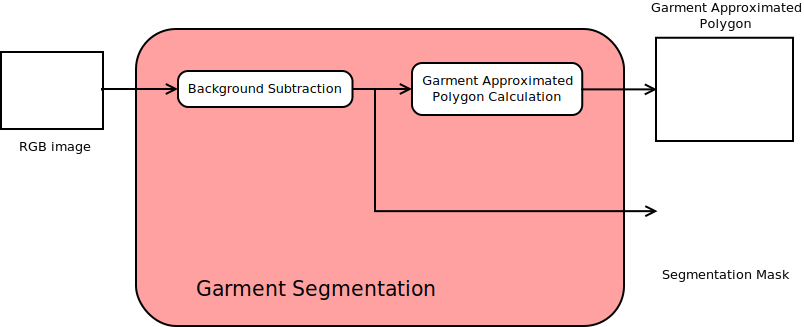
\includegraphics[width=\textwidth]
    {figures/Garment-segmentation-diagram.pdf}
    \caption[Block diagram showing an overview of the Garment Segmentation stage and its different steps.]
    {Block diagram showing an overview of the Garment Segmentation stage and its different steps. The input of this stage is an RGB image of the garment, and the outputs are the segmentation mask and the garment approximated polygon. The segmentation mask is also used as a by-product to obtain the approximated polygon.}
    \label{fig:garment_segmentation_blocks}
\end{figure}


\section{Background Subtraction}
\label{background_subtraction}

The RGB-D image obtained from the robot sensor contains both the clothing article and the table on which it rests. Therefore, after retrieving the data, a background subtraction step is required to classify whether a pixel represents the garment or the table. Figure \ref{fig:background_subtration_processes} shows an overview of the different processes involved in this step.


\begin{figure}[thpb]
    \centering
    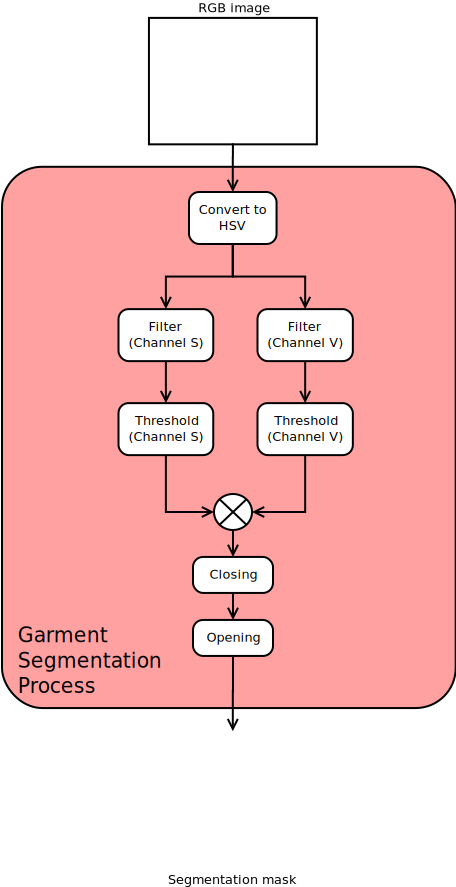
\includegraphics[width=0.6\textwidth]
    {figures/Garment-segmentation-process-diagram.pdf}
    \caption[Block diagram showing the different processes performed in the Garment Segmentation step.]
    {Block diagram showing the different processes performed in the Garment Segmentation step. The left branch of the diagram corresponds to operations performed over the Saturation (S) channel, whereas the right branch of the diagram corresponds to operations over the Value (V) channel. The Hue (H) channel of the HSV image is not used. The results of the two threshold processes are merged together with a bitwise AND operation before applying the morphological operations.}
    \label{fig:background_subtration_processes}
\end{figure}

For this purpose, many methods could have been chosen, based on both color and depth information, as discussed in section \ref{architecture:garment_segmentation}. For instance, GrabCut \cite{rother2004grabcut} was discarded for background subtraction as it requires user input to select background and foreground samples. Furthermore, it is computationally expensive compared with simple thresholding methods. As the main focus of our work is unfolding clothes, a simple color-based method was selected instead. 


We work under the assumption that the garment has been placed over a flat white surface, as opposed to the garment which is much more colorful (higher Saturation). Therefore, the RGB image is converted to the HSV space. Working in the HSV space gives us direct information about our magnitudes of interest: Saturation (S) and Value (V). We are not interested in detecting a particular color, but to detect a colored item, so HSV is a more sensible choice of color space than RGB. 

A filtering process is added to increase robustness and reduce the effect of the noise on the background subtraction. This process is achieved using a convolution with a 5x5 and $\sigma=1.1$ Gaussian kernel computed on the Saturation and Value channels of the HSV image.

Once the image is converted to the HSV color space and filtered, a thresholding operation is then applied to the filtered image, using Otsu's algorithm \cite{otsu1975threshold} to obtain the optimal threshold values. Pixels with low amount of Saturation, and high Value are classified as being part of the table, as opposed to saturated or dark pixels.

Finally, some morphological transformations are applied to the resulting mask to reduce noise due to false positives/negatives. A 5x5 square kernel is used in several closing operations, followed by a similar number of opening operations. \juansays{"Ya veremos si explicarlo"}

The output of this background subtraction step, a binary mask with background pixels represented as black and garment pixels represented as white, can be seen in Figure \ref{fig:segmentation_mask}.

%\begin{figure}[thpb]
%    \centering
%    \includegraphics[width=0.48
%    \textwidth]{figures/placeholder.png}
%    \caption{\comment{Again, I should put here a picture of the resulting mask}}
%    \label{fig:segmentation_mask}
%\end{figure}

\begin{figure}[htbp]
	\centering
    \begin{subfigure}[l]{0.49\textwidth}
	    \centering
    	\includegraphics[width=\textwidth]
    	{figures/segmentation_original.png}
    	\caption{Original RGB image}
	\end{subfigure}
	~
    \begin{subfigure}[r]{0.49\textwidth}
	    \centering
    	\includegraphics[width=\textwidth]
    	{figures/segmentation_mask.png}
    	\caption{Segmentation mask}
	\end{subfigure} 
    \caption[Original RGB image captured by the robot sensor versus the binary segmentation mask obtained after the background subtraction process.]
    {Original RGB image captured by the robot sensor versus the binary segmentation mask obtained after the background subtraction process. Black pixels represent the background, whereas white pixels represent pixels belonging to the garment.}
    \label{fig:segmentation_mask}
\end{figure}



\section{Garment Approximated Polygon Computation}
\label{segmentation_approximated_polygon}
From the binary mask obtained in the previous step (section \ref{background_subtraction}) a blob labeling algorithm is applied to detect the garment outline. This outline will be approximated to a simple polygon, and used in later stages to obtain the candidates to be a fold.

\begin{figure}[thpb]
    \centering
    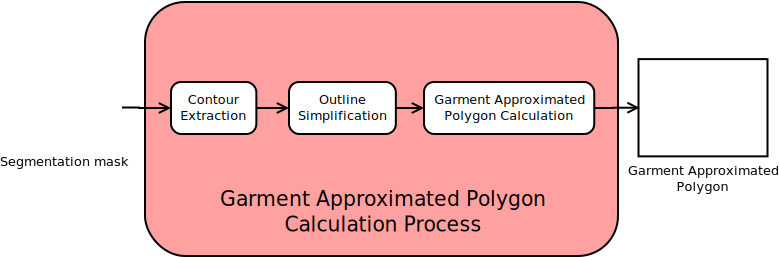
\includegraphics[width=\textwidth]
    {figures/Garment-polygon-diagram.pdf}
    \caption[Block diagram showing the different processes performed in the Garment Approximated Polygon Calculation step.]
    {Block diagram showing the different processes performed in the Garment Approximated Polygon Calculation step. The garment contour is obtained in the first process, and it is then simplified in the next processes to yield an Approximated Polygon that describes the garment.}
    \label{fig:garment_polygon_processes}
\end{figure}

The contour extraction method used is the Topological Analysis by Border Following algorithm developed by Suzuki and Abe \cite{suzuki1985topological}. It was selected as it is a widely used algorithm for connected-component labeling and countour finding. Other algorithms, such as Marching Cubes \cite{lorensen1987marching}, work under the assumption that contours are isolines\footnote{Curves along which a  function has a constant value.}, which is not the case for binary masks, so they are not suitable. Only external contours are retrieved. A simple chain approximation is then applied to reduce the number of points contained in the contours, storing only the endpoints of the different segments that describe the garment outline.

Due to noise, sometimes some small blobs appear in segmentation masks, so the outline with the largest area is selected as the garment outline. This way, those small blobs are discarded.

After obtaining the garment outline, it is futher processed, as we want to obtain a simplified description of the garment outline. This simplified description is the garment approximated polygon. We assume the fold line has a very high probability of lying in the garment polygon and, therefore, this polygon will represent all the candidate segments to be a fold. To obtain the approximated polygon, the Ramer–Douglas–Peucker algorithm \cite{ramer1972iterative, douglas1973algorithms} is applied. It is selected as it is efficient and a reliable implementation is available in the OpenCV\footnote{http://opencv.org/} libraries used to implement this work. This algorithm recursively divides the outline in segments by choosing the first and last points of the curve and drawing a line. Then, it checks whether that point is closer to that line than a threshold $\epsilon > 0$ or not. If it is closer, all points not marked to be kept can be discarded; otherwise, if it is greater than $\epsilon$, that point is marked to be kept and the procedure is repeated considering the last marked point as ending point. If there are no points left to process, the last point of the outline becomes the ending point again. The previous ending point becomes then the new starting point.

The parameter $\epsilon$ is calculated from the magnitude of the outline perimeter, considering it to be 1\% of that value. The greater this value is, the more simplified the resulting polygon will be.

Figure \ref{fig:contour_and_simplified_contour} shows a comparison between the garment contour, the garment outline and the final approximated polygon.

\begin{figure}[htbp]
	\centering
    \begin{subfigure}[l]{0.49\textwidth}
	    \centering
    	\includegraphics[width=\textwidth]
    	{figures/polygon-contour-01.png}
    	\caption{Garment Contour}
	\end{subfigure}
	~
    \begin{subfigure}[c]{0.49\textwidth}
	    \centering
    	\includegraphics[width=\textwidth]
    	{figures/polygon-outline-01.png}
    	\caption{Garment Outline}
	\end{subfigure}
	~
    \begin{subfigure}[r]{0.49\textwidth}
	    \centering
    	\includegraphics[width=\textwidth]
    	{figures/polygon-approx-01.png}
    	\caption{Garment Approximated Polygon}
	\end{subfigure} 
    \caption[Garment Contour, Garment Outline and Garment Appoximated Polygon.]
    {Garment Contour, Garment Outline and Garment Appoximated Polygon. The Garment Contour contains all the points obtained from the segmentation mask. In the Garment Outline, points belonging to the same straight line are simplified and only the start and end points of the segment are used to represent it. After the Ramer-Douglas-Peucker algorithm is applied, a polygon with a low number of edges is obtained, which is used as Garment Approximated Polygon. }
    \label{fig:contour_and_simplified_contour}
\end{figure}

	\chapter{Garment Analysis}
\label{garment_analysis}

This chapter explains in detail the gament analysis that our algorithm performs to the garment data previously segmented. The contour of the garment is extracted, and a Watershed segmentation algorithm is applied to find the different overlapped patches.

\section{Contour extraction}
From the mask obtained in the previous step (section \ref{garment_segmentation_mask}) a blob labeling algorithm is applied to detect the garment outline. This outline will be used in later steps to obtain the candidates to be a fold.

The contour extraction method used is a Topological Analysis by Border Following algorithm developed by Suzuki and Abe\comment{[ref to suzuki85]}. This is a widely used algorithm for connected-component labeling and countour finding. Only external contours were retrieved. A simple chain approximation was then applied to reduce the number of points that describe the contours, storing only the endpoints of the different segments.

Due to noise, sometimes some small blobs appear in segmentation masks, so the extracted contour with the highest area was selected as garment. This way, those small blobs were discarded.

After obtaining the garment contour, it is processed, as we want to obtain a further simplified garment outline. We assume the fold line has a very high probability of lying in the garment outline. Therefore, this contour will represent all the candidate segments that \comment{could be folds.} The Ramer–Douglas–Peucker algorithm \comment{[ref to article]} is applied to obtain the simplified outline. This algorithm recursively divides the contour in segments by choosing the \comment{...}

\section{Watershed segmentation}

Watershed is a segmentation algorithm that considers a greyscale image as a topological surface where high intensity pixels correspond to peaks and hills, and low intensity pixels are equivalent to valleys. The algorithm fills the surface pouring water at each isolated valley. As the water level rises, the water from different sources will start to merge. To prevent them from merging, the algorithm constructs barriers at the merging regions, and continues this process of adding water and building barriers until all the peaks have been flooded. The resulting barriers are the segmentation result, where each region enclosed correspond to a segmented item.

\begin{figure}[thpb]
    \centering
    \includegraphics[width=0.7
    \textwidth]{figures/placeholder2.png}
    \caption{\comment{(Here it would be great to add a figure of the example, such as opencv's coins)}}
    \label{fig:watershed_example}
\end{figure}


In the context of this work, the Watershed segmentation algorithm is applied to the depth image of the garment to locate the different parts that are overlapping each other. This regions are related to folded parts, that rest on top of other parts of the garment. 

As in practise flooding using local minima as makers leads to over- segmentation, an enhanced version of this algorithm allows the user to specify other criteria for selecting the seed points. The gradient of the greyscale depth-image was calculated for this work, and regions where the gradient has a low value were selected. These regions correspond to homogeneous and continous regions, which are good candidates to be used as markers.

To prepare it for the Watershed segmentation, the depth image was normalized and converted to a greyscale image. A denoising step was also performed, using a total variation filter \comment{(ref chambolle)}, to produce a smoother image, while maintaining the edges sharp. The total variation filter works by minimizing the integral of the norm of the image gradient. As a result of this filter, piecewise-constant images ("cartoon-like" images) are obtained.

The different garment regions obtained with watershed were labeled and used as input for the next step. Figure \ref{fig:watershed_labels} shows the result of this process.

\begin{figure}[thpb]
    \centering
    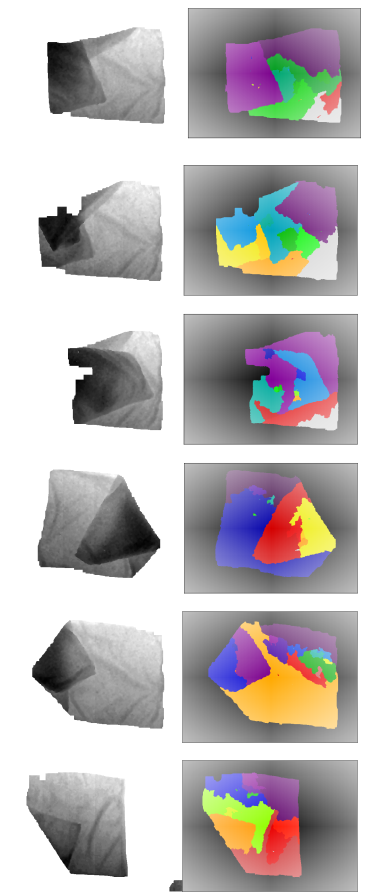
\includegraphics[width=0.38\textwidth]{figures/colour_garment.pdf}
    \caption{On the left side, the grayscale images are shown. The grey level is related to the height of the point as detected by the RGB-D sensor. On the right side, the labeled image returned by watershed algorithm is presented, where each color represents a region of similar height.}
    \label{fig:watershed_labels}
\end{figure}
	\chapter{Garment Pick and Place Points}
\label{pick_and_place}
This chapter explains the last stage of our algorithm, in which the pick and place points required for unfolding the current fold are determined. These points will be later sent to the humanoid robot to perform the unfolding operation. This stage has as input the clustered depth map obtained in the clustering stage (described in chapter \ref{garment_clustering}), and the garment approximated polygon (calculated in section \ref{segmentation_approximated_polygon}). Figure \ref{fig:garment_pnp_points_blocks} shows the block diagram of the different steps that are performed in this stage.

\begin{figure}[thpb]
    \centering
    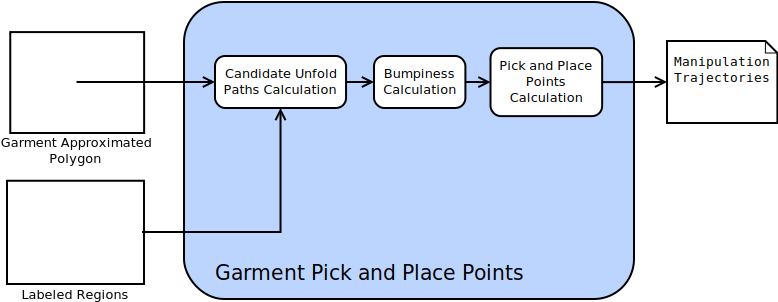
\includegraphics[width=\textwidth]
    {figures/Garment-pnp-points-diagram.pdf}
    \caption[Block diagram showing an overview of the Garment Pick and Place Points stage and its different steps.]
    {Block diagram showing an overview of the Garment Pick and Place Points stage and its different steps. The inputs for this stage are the garment approximated polygon, obtained in the Garment Segmentation stage, and the labeled cluster regions, obtained in the Garment Depth Map Clustering stage. After the analysis of these inputs, the most suitable manipulation trajectories are output to the robot to perform the unfolding action.}
    \label{fig:garment_pnp_points_blocks}
\end{figure}

\section{Candidate Unfold Paths}
\label{pnp:unfold_paths}

Based on the assumption that when a garment has an overlapping fold, the fold line will rest on the garment contour, and the folded surface will have lower depth values (i.e. closer to the depth sensor), the next step in our algorithm is to create a set of paths from the highest point of the garment to the midpoint of each contour segment. These paths will be later analyzed using the clusters previously found in the depth image to select the path with less height variation.

To find the highest point in the garment, the clusters previously found with the Watershed algorithm are averaged using the median value for each cluster. Then, the region with the lowest depth value, which is closest to the camera and therefore highest in the garment, is selected as overlapping fold based on the previous assumption. The centroid of the selected cluster is the point selected as the highest point. Using this method instead of selecting directly the highest point from the depth image increases the robustness of the algorithm against outliers and noise present in the depth image.

The midpoint of each segment of the garment approximated polygon is then calculated, and a set of paths departing from the highest point and arriving to the midpoints is created.

These paths are checked so that they are located entirely inside the garment. Paths that go outside the garment approximated polygon are considered invalid. Figure \ref{fig:candidate_paths} shows both the initial paths set and the unfold candidate paths set, without the invalid paths.


\begin{figure}[htbp]
	\centering
    \begin{subfigure}[l]{0.49\textwidth}
	    \centering
    	\includegraphics[width=\textwidth]
    	{figures/paths_candidate.png}
    	\caption{Set of candidate paths}
	\end{subfigure}
	~
    \begin{subfigure}[r]{0.49\textwidth}
	    \centering
    	\includegraphics[width=\textwidth]
    	{figures/paths_valid.png}
    	\caption{Set of valid paths}
	\end{subfigure} 
    \caption[Initial candidate paths and valid set of paths.]
    {The left image displays the set of initial candidate paths (green lines) to be used as unfolding directions. These paths are generated starting at the centroid of the highest region, represented with a magenta circle, and ending at the midpoint of each of the edges of the approximated garment polygon, shown in red lines. These paths are filtered, and the resulting valid paths, that do not cross the outer approximated polygon, are shown in the right figure.}
    \label{fig:candidate_paths}
\end{figure}


\section{Bumpiness}
\label{pnp:bumpiness}
Each of the candidate paths calculated using the method explained in the previous section has to be analyzed in this step to determine the best unfolding path. 

We can represent each of the $n$ candidate paths obtained as a 2D parametric line ($\mathbb{R} \to \mathbb{R}^2$) depending on a parameter $r$, the radial distance to the highest point:

\begin{equation}
\textrm{path}(r) = \left[u(r), v(r)\right]
\end{equation}

Where $u$ and $v$ are pixel coordinates in the image frame of reference.

Prior to the analysis, each of the paths of length $L$ is discretized in segments with a constant length $l$. The depth image $\mathcal{D}(u,v)$ is sampled at those discrete points. This results in $n$ ordered sets $S=\{ s_1,...,s_m\}$ of depth samples to be analyzed, where:


\begin{equation}
s_i = \mathcal{D}(path(i \cdot l)), \quad  i=0,1,2,..., m
\end{equation}

As the different paths may differ in length $L$, the amount of sampled points ($m=${\Large$\lfloor\frac{L}{l}\rfloor$}) will be different for each path. Figure \ref{fig:paths_with_bumpiness} shows the sample set $S$ corresponding to each candidate path for a certain garment example.

The differences in depth between the overlapping fold region and the rest of the clothing article are assumed to be greater than the diferences in depth within the fold region points. Under that assumption, the metric to evaluate the best path is a \textit{bumpiness} value \textit{B}, which is calculated by penalizing the changes in depth along each of the $n$ candidate sample sets $S$, as shown in Equation \ref{eq:bumpiness}.

\begin{equation}\label{eq:bumpiness}
B = \sum_{i=2}^{m} | s_i- s_{i-1} | 
\end{equation}

The candidate set with the lowest bumpiness value, which corresponds to the path with the least and smallest height changes, is selected as the unfold direction, as shown in Figure \ref{fig:paths_with_bumpiness}.

\begin{figure}[thpb]
    \centering
    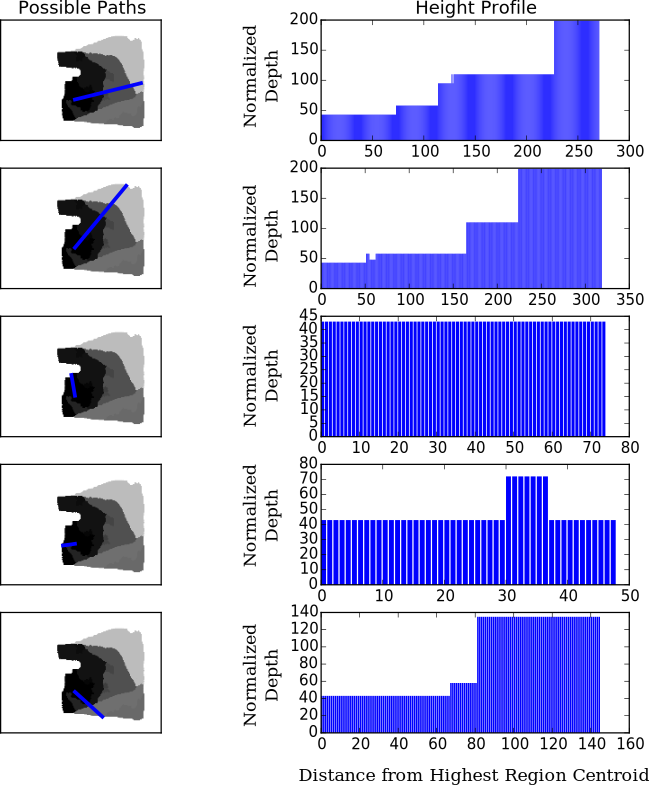
\includegraphics[width=\textwidth]{figures/candidate_paths.pdf}
    \caption[Bumpiness along several candidate paths.]
    {On the left side, the candidate paths are shown. On the right side, the height profile of each path is shown. Note that the depth sensor computes the distance to the object from itself, so that a low value in the bar plot means a closer object to the sensor, and therefore it is a region with more height with respect to the table. The highlighted path is the one with the lowest value of bumpiness, and it is selected as suitable unfolding path.}
    \label{fig:paths_with_bumpiness}
\end{figure}

\section{Pick and Place Points}
\label{pnp:pick_and_place}
Once the most promising path for unfolding has been identified, the last step is to obtain pick and place points for the robot to perform the unfold action. Due to the absence of a cuantitative metric for determining the suitability of those points, the point selection criteria has been selected using intuition from all possible choices.

The selected grasping point for the picking action is located at the intersection between the unfolding path direction line and the highest garment region border. This point is obtained by calculating the intersection between the selected path line and the highest region contour. This operation results in two intersection points, from which the furthest to the garment border is selected.

The other point is used as axis for a point reflection. To find the placing point, a reflection transformation is applied to the picking point using the aforementioned point as axis. Figure \ref{fig:directions} shows the unfold directions for several clothes, departing at the picking points and arriving to the placing points.

\begin{figure}[thpb]
    \centering
    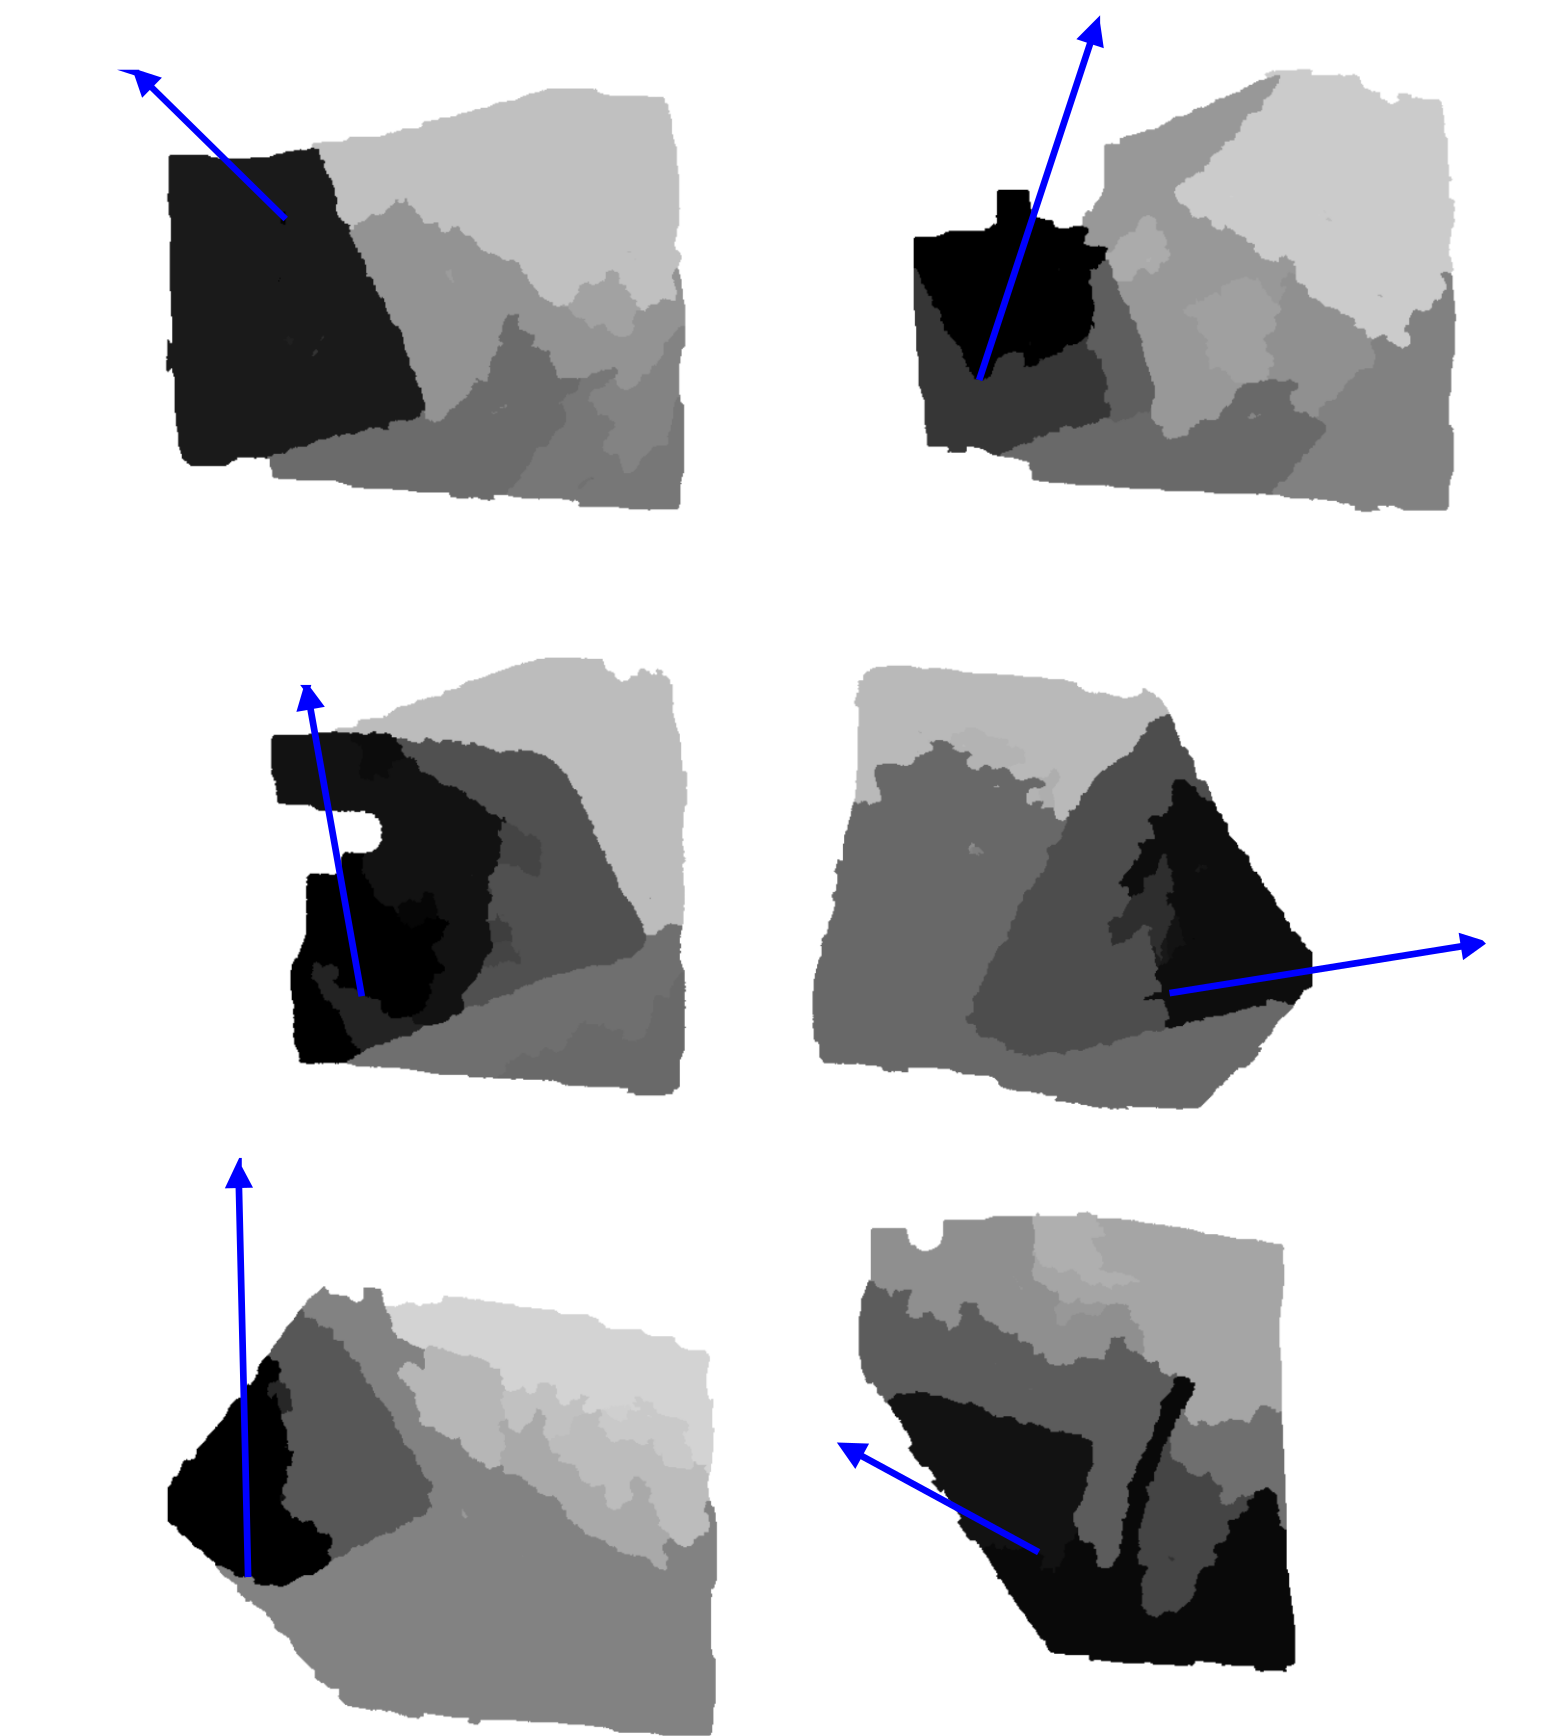
\includegraphics[width=\textwidth]
    {figures/directions.pdf}
    \caption[Final directions calculated for each garment provided to the system.]
    {Final directions calculated for each garment provided to the system. Each arrow departs where the robot should pick the fold and arrives where it should be placed. Darker regions represent regions that are closer to the camera, whereas lighter regions represent regions of the garment further from the camera.}
    \label{fig:directions}
\end{figure}

\comment{Lorem ipsum dolor sit amet, consectetur adipiscing elit. Donec a diam lectus. Sed sit amet ipsum mauris. Maecenas congue ligula ac quam viverra nec consectetur ante hendrerit. Donec et mollis dolor. Praesent et diam eget libero egestas mattis sit amet vitae augue. Nam tincidunt congue enim, ut porta lorem lacinia consectetur. Donec ut libero sed arcu vehicula ultricies a non tortor. Lorem ipsum dolor sit amet, consectetur adipiscing elit. Aenean ut gravida lorem. Ut turpis felis, pulvinar a semper sed, adipiscing id dolor. Pellentesque auctor nisi id magna consequat sagittis. Curabitur dapibus enim sit amet elit pharetra tincidunt feugiat nisl imperdiet. Ut convallis libero in urna ultrices accumsan. Donec sed odio eros. Donec viverra mi quis quam pulvinar at malesuada arcu rhoncus. Cum sociis natoque penatibus et magnis dis parturient montes, nascetur ridiculus mus. In rutrum accumsan ultricies. Mauris vitae nisi at sem facilisis semper ac in est.}


	\chapter{Experiments and results}
\label{experiments_and_results}

\section{Experiments}
\label{experiments}

This section is devoted to explain the experiments performed using the algorithm presented in this thesis. It includes the implementation details, the experimental setup and the experiments themselves.

\subsection{Implementation details}
The software implementation has two main parts. The first one is in charge of communication with the sensor with the objective of extracting the depth data. This communication is performed using YARP\footnote{\url{http://www.yarp.it}}. YARP is a middleware software library \comment{(framework)} that leverages many common tasks required for a robot to work. Those tasks include actuator control and command, communications with the robot and between software parts, and accessing to different common sensors, such as depth sensors.

The second one is the implementation of the unfolding pipeline (algorithm). This implementation was executed using Python\footnote{\url{http://www.python.org}} as our language of choice. Python is a programming language that allows a quick development of prototype software, and that counts with a large collection of external libraries \comment{(modules)} to perform several tasks, from math calculations to computer vision. Our implementation is based on tho different computer vision libraries: OpenCV\footnote{\url{http://www.opencv.org}} and Scikit-image\footnote{\url{http://scikit-image.org}}, since during the development of this work several algorithms were evaluated. OpenCV is used for \comment{the basic vision stuff} and Scikit-image for more advanced algorithms such as Watershed \footnote{\url{http://scikit-image.org/docs/dev/auto_examples/plot_watershed.html}} and other superpixel-based clustering methods. Both libraries are compatible \comment{and working with both of them is not a problem}.

The whole unfolding algorithm implementation is Open Source, and is available online\footnote{\url{https://github.com/roboticslab-uc3m/textiles}}.

\subsection{Data adquisition}
\label{data_adquisition}

The starting point of our algorithm is the data adquisition process. Data is obtained as a point cloud from a ASUS Xtion Pro Live sensor. Then, data is converted to a depth map image for its later analysis. 

This conversion is done by simply using the z component of each point as the depth value for each pixel of the depth image. This depth image could also be recovered from the point cloud using the instrinsic and extrinsic paramters of the sensor. But, as the sensor is placed on top of the garment, perpendicular to the surface on which the clothing article rests, both methods yield almost very similar results.

\begin{figure}[thpb]
    \centering
    \includegraphics[width=0.7
    \textwidth]{figures/placeholder2.png}
    \caption{\comment{Here I should put a nice figure of the point cloud and the depth image}}
    \label{fig:point_cloud_and_depth_image}
\end{figure}

The RGB values are also recorded for each depth image, obtaining an RBG-D image.

\subsection{Other stuff}

The final experiments using the current algorithm have been performed using an ASUS Xtion PRO LIVE at 640x480 RGB and depth streams (30 fps).
To simplify the image analysis, the sensor is placed on top of the working surface  providing a bird's eye view over the cloth folding environment, with its image plane almost parallel to the working surface.

In the present work we are using thick blankets and towels, to cope with the limitations of the resolution of the depth sensor. A set of six samples with one or two folds were presented to the system for analysis. The results are shown in Fig. \ref{directions}.
%
These results show that the algorithm generates acceptable unfolding directions.

%However, when analyzing the experimental results, one can see that the candidate paths for unfolding are created using the garment contour segment midpoint. This fact can warp the most intuitive direction, which would be the closest between the highest region and the garment contour.

According to the results, an interpolation between the best two directions could result in a better solution. The best directions for the set of clothes are shown in Fig. \ref{directions_several}. %The arrow's directions make us believe that a combined directions by averaging them could provide better results.

%\warning{In \cite{Li2015IROS}, Li et al. present a method for folding deformable objects such as clothes. }

%A final demonstration of the current algorithm has been performed using the full-size humanoid robot TEO \cite{martinez2012teo}. Depth sensor coordinates are passed to the robot root frame, and a standard pick and place operation is performed with the given points. Figure \ref{setup} depicts this scenario.

\footnote{\url{http://scikit-image.org/docs/dev/auto_examples/plot_watershed.html}} 

\section{Data adquisition}
\label{data_adquisition}

The starting point of our algorithm is the data adquisition process. Data is obtained as a point cloud from a ASUS Xtion Pro Live sensor. Then, data is converted to a depth map image for its later analysis. 

This conversion is done by simply using the z component of each point as the depth value for each pixel of the depth image. This depth image could also be recovered from the point cloud using the instrinsic and extrinsic paramters of the sensor. But, as the sensor is placed on top of the garment, perpendicular to the surface on which the clothing article rests, both methods yield almost very similar results.

\begin{figure}[thpb]
    \centering
    \includegraphics[width=0.7
    \textwidth]{figures/placeholder2.png}
    \caption{\comment{Here I should put a nice figure of the point cloud and the depth image}}
    \label{fig:point_cloud_and_depth_image}
\end{figure}

The RGB values are also recorded for each depth image, obtaining an RBG-D image.

\input{results}

\begin{figure}[thpb]
    \centering
    \includegraphics[width=0.8\textwidth]{figures/directions_several.png}
    \caption{Best directions calculated for each garment provided to the system. The direction with the smallest bumpiness value is shown in blue. The second best direction is shown in yellow. The bisector is shown in green. The arrows are for demonstrative purpose only, and their starting and ending point do not represent the pick and place point. The watershed computed regions are additionally overlaid upon the original image.}
    \label{directions_several}
\end{figure}

	\chapter{Conclusions and future work}
\label{conclusions_and_future_work}

This chapter will describe the main contributions made to the state of the art by this work. Along the development of this work and during the experiments some challenges appeared. They will be covered after the main contributions along with future work lines that address those challenges and  further improve the state of the art.


\section {Main contributions}
\label{conclusions:contributions}

This section is dedicated to explain the main contributions of this work, and develop them in detail according to the different steps in our unfolding algorithm.

The main contribution of our work is that its analysis of the garment is not dependent of a prior model. The process core resides in the segmentation of the grayscale image representing the heights. Results show that our approach is promising to be included in a complete pipeline of clothes folding.

\begin{enumerate}
	\item \textbf{Garment Segmentation:} Regarding garment segmentation, our main contribution is a segmentation stage that is independent of the shape and color of the garment. This stage works as long as the table that holds the garment is white or grey and the garment is more colorful than the table. The segmentation stage, additionally, requires no user input to label background/foreground samples.
	\item \textbf{Garment Depth Map Clustering:} Our algorithm improves existing approaches by using Watershed as clustering algoritm, so that a threshold value for labelling contiguous regions is not required. This absence of threshold value also avoids breaking similar height regions into different label regions due to large wrinkles. 
	\item \textbf{Garment Pick and Place Points:} The main contribution of this work regarding   choosing pick and place points is that the selection of those points is independent of the garment category. Previous work found in the literature required the garment category or model to be specified or learnt to have a prior knowledge of the most suitable grasping points.
\end{enumerate}

\section{Future Work}
\label{conclusions:future_work}
Some opportunities exist to further develop and improve this work, despite the presented satisfactory results. This section will introduce those current issues and possible solutions to address them, regarding each of the stages that compose our algorithm.

\begin{enumerate}
	\item \textbf{Garment Segmentation:} As our garment segmentation stage currently depends on color, it sometimes trims some areas of the garment due to ilumination or a wrong white balance of the RGB camera. This segmentation problem may result in an incorrect polygon approximation that affects the functionality of the system.
	\item \textbf{Garment Depth Map Clustering:} In general, we have found that working with a single point of view is a very limiting factor, as occlusions sometimes make folds ambiguous. As our approach does not depend on garment models, dissambiguating those situations is very challenging. For that reason, the author strongly believes that moving to an approach that uses a 3D point cloud of the garment as input data would have more information available to solve those ambiguous situations in a better way.

	\item \textbf{Garment Pick and Place Points:} While the selected points may serve as a rule-of-thumb for robotic system developers, there is no clear metric for evaluating cuantitatively the suitability of the selected points. Therefore, experimental validation through further experiments with robotic systems is required to determine whether a better pick and place strategy exists:
	
\begin{itemize}
\item For instance, the highest garment point or highest region centroid could be used as alternative to the current pick point, \comment{under the assumption that that point would correspond to an overlapped garment region not attached to the garment regions underneath}.

\item Other place points could also be chosen depending on a different criteria. For example, the place point could be calculated using the fold line as axis of symmetry, or determined based on the unfolding trajectory selected.	

\item The trajectory used to unfold the garment is a simple one, which follows a straight line connecting the pick point, a point above the pick point, a point above the place point and the place point. More elaborated trajectories, such as splines or curves, could be used instead, such the one Li et al. present in their method for folding deformable objects \cite{Li2015IROS}.

\end{itemize}
\end{enumerate}

Finally, as the experiments were performed using data gathered from a limited set of garments in our laboratory environment, the statistical relevance of the results is also limited. Future works should include the use of datasets of garments shared and used among other laboratories and research groups to promote fair benchmarking through repeatable experiments.



\bibliographystyle{apacite}
\bibliography{library}
		
\end{document}